\chapter{Двухчастотное волновое смешение в импульсном режиме}
\label{ch: q_mixing}

В данной главе будут описаны эффекты волнового смешения, возникающие при импульсной бихроматической накачке двухуровневой системы. В этих экспериментах на кубит подаются последовательности прямоугольных или близких к ним по форме импульсов. Несущие частоты этих последовательностей незначительно отстроены от резонанса кубита, длительности импульсов варьируются от $0$ до нескольких $T_1$ кубита, а промежутки между импульсами значительно превышают $T_1$. Качественная картина спектра эластичного рассеяния претерпевает значительные изменения по сравнению с непрерывной накачкой. Например, при рассеянии синхронизированных прямоугольных импульсов на частотах $\omega_{pm}$ наблюдается бесселевская динамика боковых компонент сигнала в зависимости от эффективной длительности импульса $\Omega\Delta t$. Совершенно новый физический эффект возникает при введении задержки между последовательностями импульсов. Длительность задержки должна превосходить длительность импульса для того, чтобы отдельные импульсы на частоте $\omega_+$ попадали на кубит раньше импульсов на частоте $\omega_-$ и не перекрывались с ними. При этом кардинально меняется вид спектра эластичного рассеяния. Вместо большого количества симметричных пиков мы наблюдаем лишь один дополнительный пик на частоте $2\omega_--\omega_+$. Этому эффекту можно дать простое качественное объяснение, напрямую вытекающее из свойства кубита поглощать не более чем единичный квант поля. В дополнение к этому, мы изучаем рассеяние последовательностей импульсов на трехуровневой эквидистантной системе, которая возникает при некотором значении внешнего магнитного потока, проходящего через петлю изучаемого нами потокового кубита. Помимо к двух компонент на исходных несущих частотах и одной компоненте от четырехволнового смешения, к эластичному спектру добавляется еще две компоненты, соотвествующие двухфотонным процессам, что подтверждает справедливость качественной интерпретации экспериментальных результатов. Последние два режима мы будем называть \textit{квантовым волновым смешением}, поскольку оно обладает рядом необычных свойств, обусловленных квантовостью сверхпроводникового искусственного атома. В дополнение к экспериментальным данным, в данном разделе проведен численный расчет спектра, согласующийся с экспериментом, а также дано строгое теоретическое обоснование трехпикового спектра рассеяния на двухуровневой системе и пятипикового спектра рассеяния на трехуровневой системе на основе формализма вторичного квантования.  
\section{Случай синхронных импульсов: бесселевская динамика}
\label{sec: bessels}
Для изучения импульсного смешения при помощи экспериментальной схемы \ref{fig: pulse_setup_1} необходимо запрограммировать генератор импульсов произвольной формы (AWG) так, чтобы на его выходе получить последовательность прямоугольных импульсов. Несущая частота этих импульсов $\omega_{\text{IF}}/2\pi$ может варьироваться от 0 до 100 МГц, а период импульсов $T\gg 1/\Gamma_1$ обеспечивает релаксацию кубита после импульса за время, предшествующее появлению следующего импульса. Длительности импульсов $\delta t$ также меняются произвольно, технические возможности AWG позволяют получить импульсы длительностью от 2 нс и выше. Импульсный сигнал с выхода AWG попадает на квадратурный смеситель, где смешивается с сигналом локального осциллятора, приобретая таким образом несущую частоту $\omega_{d} = \omega_{\text{LO}}\pm\omega_{\text{IF}}$, где выбор знака произволен и зависит от калибровки квадратурного смесителя. Затем сигнал направляется в криостат, попадает в волновод с искусственным атомом и рассеивается на нем.  Детектирование рассеянного сигнала осуществляется при помощи спектрального анализатора либо при помощи высокоскоростного АЦП. Во втором случае на выходе сигнал испытывает обратное преобразование частоты вниз при помощи еще одного квадратурного смесителя, после чего сигнал на частоте $\omega_{\text{IF}}$ оцифровывается, а квадратуры комплексного сигнала $I$ и $Q$ вычисляются при помощи цифрового преобразования Фурье \cite{sank2014fast}.

Сгенерировав две синхронные последовательности импульсов одинаковой длительности $\Delta t_-\!=\!\Delta t_+\!=\!\Delta t$ на частотах $\omega_+$ и $\omega_-$ описанным способом и подав их на кубит, мы измеряем спектр эластичного рассеяния, усредненный по большому количествую периодов. Это достигается установлением параметра RBW (Resolution Bandwidth) спектрального анализатора до 1 кГц и ниже, что делает время усреднения более 1 мс, тогда как период следования импульсов составляет 1-10 мкс. Очевидно, что длительности $\Delta t$ импульсов оказывают ключевое влияние на характер динамики кубита, и соответственно, определяют свойства рассеянного излучения, поэтому мы снимаем зависимости интенсивностей боковых компонент от эффективной длительности импульсов $\Omega\Delta t$.
Результат этих измерений изображен на Рис \ref{fig: Bessels}. 
\begin{figure}\label{fig: Bessels}
\centering
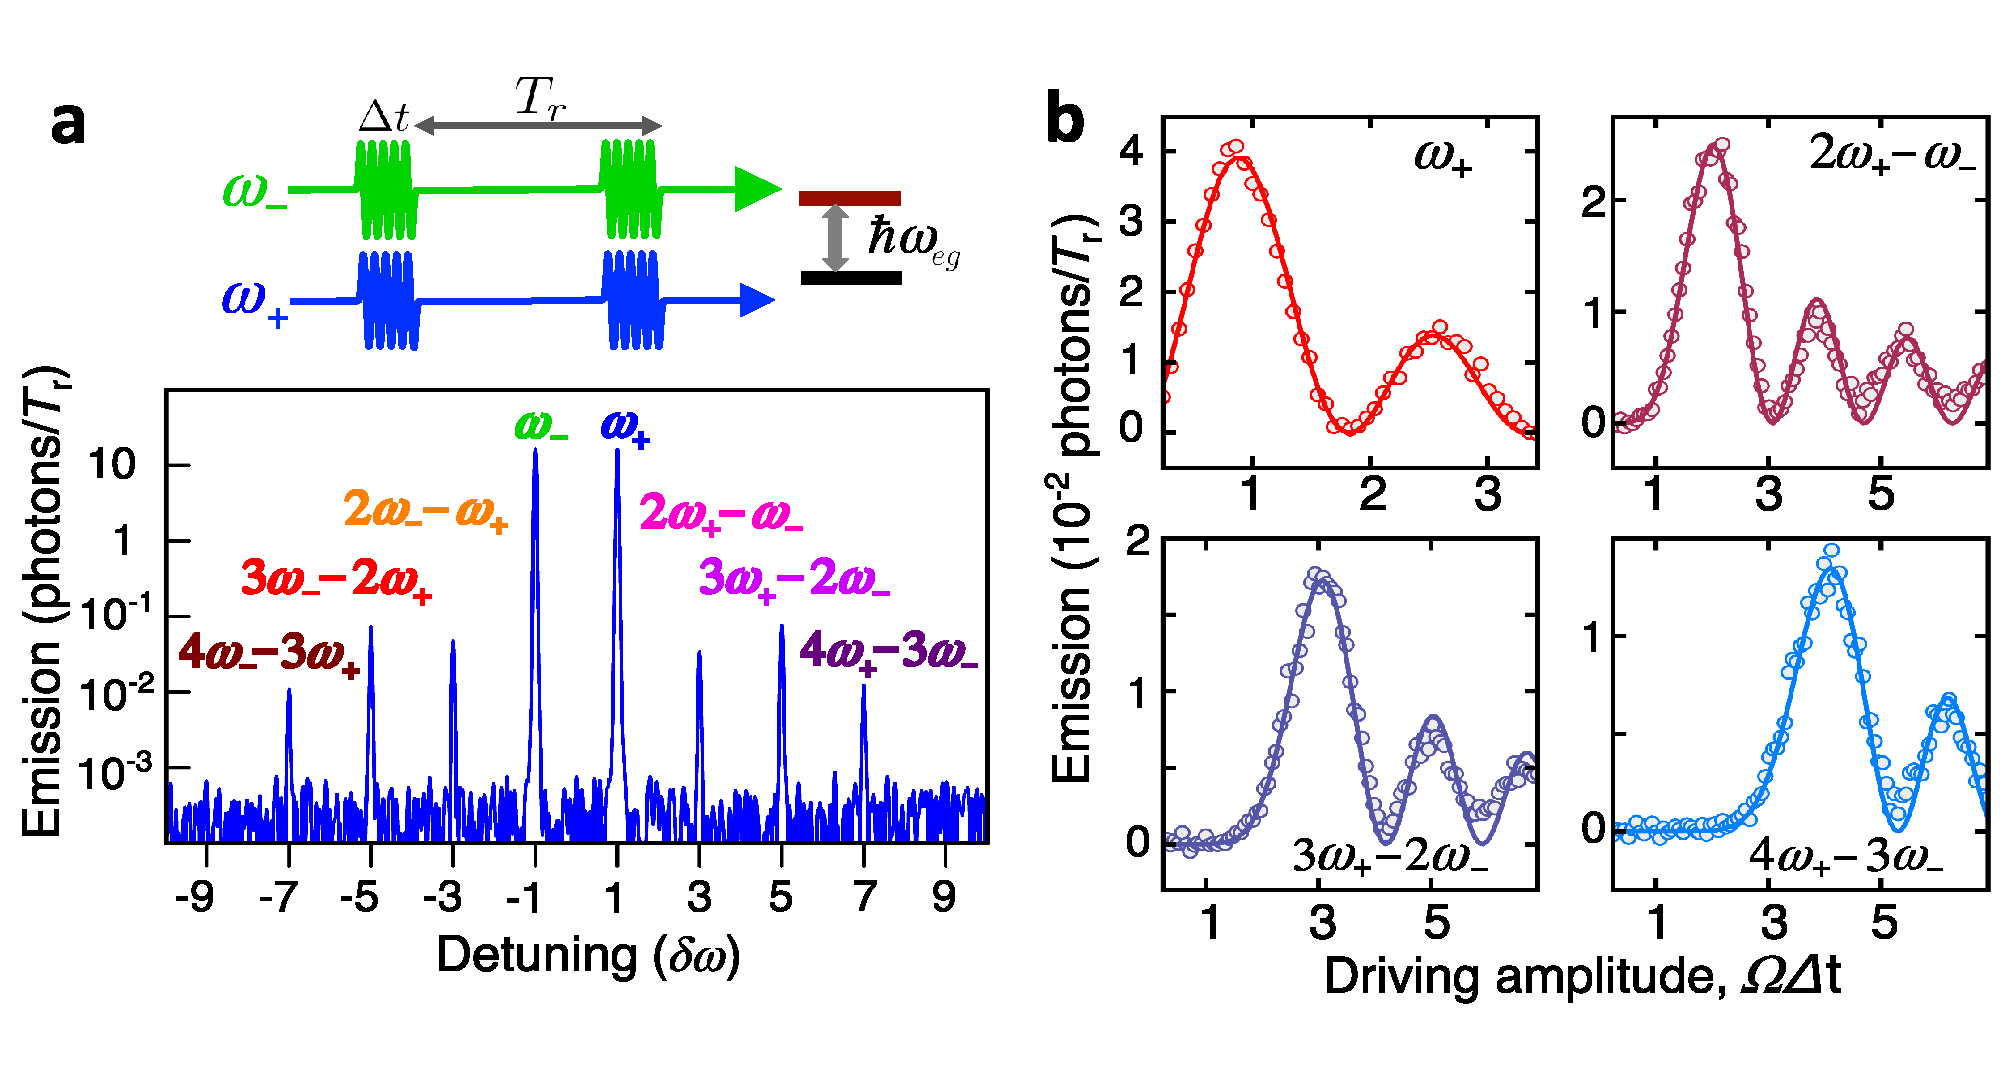
\includegraphics[width=1\textwidth]{Bessels.pdf}
\caption[Зависимость интенсивности боковых компонент от длительности импульсов $\Delta t$ бихроматической накачки]{Зависимость интенсивности боковых компонент от длительности импульсов бихроматической накачки. (a) Последовательность управляющих импульсов длительностью $\Delta t=2$~нс с периодом $T_r=1$~мкс и часть спектра эластичного рассеяния c когерентыми пиками. (б) Измеренные зависимости потока фотонов в пике от угла поворота $\zeta_{2p+1}(\Omega \Delta t). $. Точками показаны результаты измерений, сплошные линии соответствуют выражениям $J^2_{2p+1}(2\Omega\Delta t)/4$, описывающим эксперимент без подгоночных параметров.}
\end{figure} 
Этот результат достаточно просто объясняется динамикой кубита под воздействием классического поля. Для динамики кубита под действием двух классических импульсов можно получить следующее выражение:
\begin{equation}
	\braket{\sigma_-} = -\frac{1}{2}\sin(2\Omega\Delta t \cos\delta\omega t), 
\end{equation}
которое раскладывается в ряд по бесселевским функциям согласно соотношению Ангера-Якоби:
\begin{equation}
	\langle \sigma^- \rangle = -\sum_{k=-\infty}^\infty (-1)^k J_{2k+1}(2\Omega \Delta t) \cos[(2k+1)\delta\omega t],
\end{equation}
и усреднение спектральных компонент $\langle \sigma^-_{2k+1}\rangle$ с определенным набегом фазы $(2k+1)\delta \omega t$ дает:
\begin{equation}
	\langle \sigma_{2k+1}^-\rangle = \frac{(-1)^k}{2}J_{2k+1}(2\Omega t),
	\label{sclass_spectr} 
\end{equation} 
что соответствует экспериментально представленным зависимостям на Рис.~\ref{fig: Bessels}. Данный результат можно представить как разложение осцилляций Раби, которые наблюдались бы при $\delta\omega =0$, по разным спектральным компонентам.

Вывод результата \eqref{sclass_spectr} достаточно прост и не требует квантовомеханического описания поля, но тем не менее, он не иллюстрирует сущность наблюдаемого волнового смешения, в частности, не выделяет индивидуальный вклад различных многофотонных процессов в излучение и связь с фотонной статистикой излучаемого света. Более того, полуклассическая картина не выявляет физического происхождения ограниченного количества спектральных компонент, которые мы будем наблюдать для случая квантового волнового смешения двух последовательностей импульсов бихроматической накачки с задержкой. Поэтому мы получим бесселевскую динамику также при помощи рассмотрения эволюции кубита под воздействием двух квантованных мод поля, описывающихся операторами $a_\pm$ и $a_\pm^\dag$, взаимодействующих с кубитом. Как мы увидим далее, этот формализм позволяет описать не только случай синхронных импульсов, характеризующийся рассмотренной выше бесселевской динамикой, но и случай последовательных неперекрывающихся во времени импульсов, где спектр кардинально отличается от рассмотренного выше режима. Для начала, выпишем и обсудим несколько известных результатов, касающихся взаимодействия для одной моды внутри волновода и кубита, связанного с этим волноводомё. 

Будем рассматривать двухуровневый атом с основным и возбужденными состояниями $\ket{g}$ и $\ket{e}$ и энергией $\hbar \omega_0$, взаимодействующий с квантованным полем на частоте $\omega$. Эта система может характеризоваться гамильтонианом, записанным в представлении взаимодействия:
\begin{equation}
	H = i\hbar g (a^\dag \sigma^-  e^{i\delta\omega t} - a \sigma^+  e^{-i\delta\omega t}),
	\label{Hqint}
\end{equation}
где $\hbar g$ --- энергия связи между полем и атомом, $\delta\omega = \omega - \omega_0$ --- отстройка, которую мы считаем достаточно малой, $\sigma^{+} = \ket{e}\bra{g}$ и $\sigma^{-} = \ket{g} \bra{e}$ --- повышающий и понижающий операторы для состояний атома, а $a^\dag$ ($a$) --- операторы рождения и уничтожения фотонных состояний $|n\rangle$  на частоте $\omega = \omega_0 + \delta\omega$. 
Эволюция системы на коротком временном интервале $\Delta t \ll \delta\omega^{-1}$ описывается оператором $U(t',t) = \exp(-\frac{i}{\hbar} H_t \Delta t)$, где $H_t$ --- гамильтониан в момент времени $t$, $\Delta t = t'-t$. Оператор эволюции может быть разложен в бесконечный ряд по формуле:
\begin{equation}
	\begin{split}
		U(t',t) = 1 + 
		\eta (a^\dag s^- - a s^+ ) 
		-\frac{\eta^2}{2!} (a a^{\dag} s_{e} + a^{\dag}a s_{g} ) -
		\frac{\eta^3}{3!} (a^{\dag} a a^\dag s^- - a a^{\dag}a s^+)+... ,
	\end{split}
	\label{ut}
\end{equation}
где $\eta = g\Delta t$ и $s^\pm$ --- зависящие от времени операторы $s^+(t) = \sigma^+ e^{-i\delta\omega t}$ и $s^-(t) = \sigma^- e^{i\delta\omega t}$. 
Данный ряд можно записать в более простом виде: 
\begin{equation}
	\begin{split}
	U(t',t) =  \cos{\big(\eta \sqrt{a^\dag a}\big)} s_g &+ \cos{\big(\eta \sqrt{a a^\dag}\big)} s_e - \\
	&- \frac{a s^+}{\sqrt{a^\dag a}} \sin{\big(\eta \sqrt{a^\dag a}\big)} + \frac{a^\dag s^-}{\sqrt{a a^\dag}} \sin{\big(\eta \sqrt{a a^\dag}\big)},
	\end{split}	
\end{equation}
где $s_e = s^+ s^-$ and $s_g = s^- s^+$. Преобразуя далее, имеем:
\begin{equation}
	\begin{split}
		U(t',t) = \sum_{n=0}^{\infty} \Big[  \cos{\big(\eta \sqrt{n}\big)} &|n\rangle\langle n| s_g + \cos{\big(\eta \sqrt{n+1}\big)} |n\rangle\langle n| s_e - \\ 
		&|n\rangle\langle n+1| s^+ \sin{\big(\eta \sqrt{n}\big)} + |n+1\rangle\langle n| s^- \sin{\big(\eta \sqrt{n+1}\big)} \Big].	
	\end{split}
	\label{ut}
\end{equation}
В частности, для начального состояния $\Psi(t) = \ket{g,n}$, эволюция в результате приводит к состоянию $\Psi(t')=\cos(\eta \sqrt{n}) \ket{g,n}-e^{-i\delta\omega t} \sin(\eta \sqrt{n}) \ket{e, n-1}$. Мы будем рассматривать эволюцию под воздействием сильного когерентного излучения  $\ket{\alpha}$, где действительное $\alpha \gg 1$.

Когда $\Psi(t) = |g,\alpha\rangle$, эволюция упрощается:  
\begin{equation}
	\Psi(t') \approx \cos\frac{\theta}{2} \ket{g, \alpha} - e^{-i\delta\omega t} \sin \frac{\theta}{2} \ket{e, \alpha}
	\label{Rb}
\end{equation}
где $\theta = 2\eta\alpha$, $\alpha = \sqrt{\langle n\rangle}$ и $|\alpha'\rangle = \Big(1-e^{-|\alpha |^2}\Big)^{-1/2}\sum_{n=1}^\infty |n-1\rangle\langle n|\alpha\rangle $. В интересующем нас случае $\alpha \gg 1$ и поэтому поглощение одного фотона атомом эффективно не меняет состояние: $\ket{\alpha'} \approx \ket{\alpha}$. Мы можем переписать состояние в \eqref{Rb} как: 
$\Psi(t') \approx (\cos\frac{\theta}{2} |g\rangle - e^{-i\delta\omega t}\sin \frac{\theta}{2} |e\rangle)\otimes |\alpha\rangle$. После прохождения импульса, фотонное поле полностью излучается ($|\alpha\rangle \rightarrow |0\rangle$) и состояние системы приобретает вид:   
\begin{equation}
	\begin{split}
		\Psi' = \bigg(\cos\frac{\theta}{2} |g\rangle - e^{-i\delta\omega t}\sin \frac{\theta}{2} |e\rangle\bigg)\otimes |0\rangle 	
	\end{split}
	\label{Rb2}
\end{equation}
и для среднего значения оператора понижения с учетом фазы имеем:
\begin{equation}
	\langle s^+ \rangle = -\frac{\sin{\theta}}{2}.
	\label{sp}
\end{equation}

Атом, находящийся в состоянии суперпозиции (при $\theta \neq M \pi$, где $M$ это целое число) приобретает фазу $\delta\omega t$ из начальной когерентной волны \cite{Astafiev2010resonance,abdumalikov2011dynamics} и затем излучает в волновод суперпозицию нуля и одного фотона. 
%This can be exemplified by analysing the evolution $U(t')\Psi' = (\cos\frac{\theta}{2} |g, 0\rangle - ie^{i\phi}(\sin\frac{\theta}{2}\cos\frac{\theta'}{2} |e, 0\rangle - i\sin\frac{\theta}{2}\sin\frac{\theta'}{2} |g, 1\rangle)$, where $\theta' = 4 g t'$. 
Полезно проанализировать эволюцию состояния $\Psi'$ из уравнения \eqref{Rb2} под действием оператора (\ref{ut}). Когда накопленный угол $\eta = \frac{\pi}{2}$, % $U_{ap} = 1-i (s^- a^\dag+s^+ a)$ 
\begin{equation}
	U_{ap} = |0\rangle\langle0| \sigma^-\sigma^+ + e^{i\delta\omega t} |1\rangle\langle 0 | \sigma^-
	\label{Uap}
\end{equation} 
и суперпозиция атомного состояния перетекает в суперпозицию однофотонного поля на частоте $\omega$ следующим образом:    
\begin{equation}
	%\begin{split}
	U_{ap} \bigg[ \bigg(\cos{\frac{\theta}{2}} |g\rangle - e^{-i\delta\omega t} \sin{\frac{\theta}{2}} |e\rangle\bigg) \otimes |0\rangle \bigg] =  
	|g\rangle \otimes \bigg(\cos{\frac{\theta}{2}} |0\rangle - \sin{\frac{\theta}{2}} |1\rangle\bigg).
	\label{sps}
\end{equation} 
Мы введем однофотонный оператор рождения $b^+ = |1\rangle\langle0|$  на частоте $\omega$ и тогда
\begin{equation}
	\langle b^+\rangle = -\frac{1}{2}\sin\theta. 
	\label{bp}
\end{equation}
Уравнения (\ref{sp} - \ref{bp}) теперь могут быть переписаны при помощи $b$-операторов и важным следствием этого является тот факт, что состояние суперпозиции в атоме переходит в когерентное однофотонное поле при замене $s^+ \rightarrow b^+$ и $s^- \rightarrow b^-$, где введен оператор $b^- = |0\rangle\langle 1|$. 

%Importantly, the generated field is coherent, however essentially different from the classical coherent state $|\alpha \rangle=e^{-{|\alpha|^2}/{2}}\sum_{n=0}^{\infty}\alpha^n /\sqrt{n!} |n\rangle$ and $\alpha = \sqrt{\langle n\rangle}$ consisting of an infinite number of photon states. 

Классическое когерентное и однофотонное состояния могут быть представлены в похожей форме: 
\begin{subequations}
	\begin{alignat}{2}
		|&\alpha\rangle = & A \bigg( & |0\rangle + \alpha |1\rangle + \frac{\alpha^2}{\sqrt{2!}} + ...\bigg)\\
		|&\beta\rangle = & B \big( & |0\rangle + \beta |1\rangle\big),
	\end{alignat}
\end{subequations}
где $A=\exp{(-|\alpha|^2/2)}$ и $B=(1+|\beta|^2)^{-1/2}$. В частности, для когерентного состояния из уравнения \eqref{sps}, $\beta = -\tan \theta/2$ и $B=\cos \theta/2$. 

На основе вышеизложенного, гамильтониан~\eqref{Hqint} может быть эквивалентным образом представлен при помощи однофотонных операторов рождения и уничтожения следующим образом: 
\begin{equation}
	H' = i\hbar g (b^+ a - b^- a^\dag),
	\label{Hqintb}
\end{equation}
подразумевая, что $b$-операторы описывают фотоны, излученные атомом с фазой $\delta\omega t$ и потому удовлетворяют соотношениям, типичным для $s$-операторов: $b^+b^- = |1\rangle\langle 1|$, $b^-b^+ = |0\rangle\langle 0|$, $b^+b^+ = 0$, $b^-b^- = 0$. 

В дополнение, можно упростить уравнение~(\ref{ut}) для случая достаточно коротких импульсов достаточно сильного когерентного поля следующим образом: 
%\begin{equation}
%\begin{split}
%	U(t',t) = \sum_{n=0}^{\infty} &\cos{\big(\eta \sqrt{n}\big)} |n\rangle\langle n| b^-b^+ + \cos{\big(\eta \sqrt{n+1}\big)} |n\rangle\langle n| b^+b^- -\\ 
%	&\sin{\big(\eta \sqrt{n}\big)} |n-1\rangle\langle n| b^+ + \sin{\big(\eta \sqrt{n+1}\big)} |n+1\rangle\langle n| b^-.	
%\end{split}
%\label{ut}
%\end{equation}
%
%\begin{equation}
%	U(t',t) = \cos{\big(\eta \sqrt{a^\dag a}\big)} b^-b^+ + \cos{\big(\eta \sqrt{a a^\dag}\big)} b^+b^- -
%	\frac{a b^+}{\sqrt{a^\dag a}} \sin{\big(\eta \sqrt{a^\dag a}\big)} + \frac{a^\dag b^-}{\sqrt{a a^\dag}} \sin{\big(\eta \sqrt{a a^\dag}\big)}.	
%\end{equation}
%
\begin{equation}
	U(t',t) \approx \cos{\big(\eta \sqrt{a^\dag a}\big)} + (a^\dag b^- - a b^+) \frac{\sin{\big(\eta \sqrt{a^\dag a}\big)}}{\sqrt{a^\dag a}}.	
	\label{u1}
\end{equation}

%\begin{equation}
%\langle b^+_{2k+1} \rangle = \frac{(-1)^k}{2}  J_{2k+1}[2\Omega\Delta t]. 
%\end{equation}

Вернемся к случаю импульсной бихроматической накачки. Для этого, мы рассматриваем два непрерывных когерентых поля $|\alpha_{-}\rangle_-$ и $|\alpha_{+}\rangle_+$, где $\alpha_{\pm}$ --- действительные комплексные амплитуды поля. Гамильтониан \eqref{Hqintb} принимает вид:
\begin{equation}
	%H = \hbar g \sum\limits_{k=0}^{\infty} (\sigma^+ a_{\pm(2k+1)} + \sigma^- a^\dag_{\pm(2k+1)}),
	%H = \hbar g (\sigma^+ a_{1} + \sigma^+ a_{-1}+c.c.),
	%H = \hbar g (\sigma^+ a_{1} + \sigma^- a^\dag_{1} + \sigma^+ a_{-1} + \sigma^-a^\dag_{-1}),
	H_{2} = i\hbar g(s_-^-a^\dag_{-} - s_-^+ a_{-}  + s_+^- a^\dag_{+} + s_+^+ a_{+} ) ,
	\label{Hm}
\end{equation}
где $a^\dag_\pm$ ($a_\pm$) --- операторы рождения (уничтожения) фотона на частотах $\omega_\pm$, $s_+^\pm = \sigma e^{\mp i\delta\omega t}$, $s_-^\pm = \sigma e^{\pm i\delta\omega t}$ и $\hbar g$ обозначает константу связи кубита к модам. Оператор эволюции, соответствующий гамильтониану ~(\ref{Hm}) может быть расписан аналогично уравнению~(\ref{ut}), однако, каждое слагаемое содержит последовательные комбинации операторов $s_\pm^- a^\dag_{\pm}$ и $s_\pm^+ a_{\pm}$. Мы можем переписать гамильтониан через $b$-операторы при помощи подстановки $s_\pm^+ \rightarrow b_\pm^+$ and $s_\pm^- \rightarrow b_\pm^-$,  
\begin{equation}
	H = i \hbar g\big(b_-^+ a_{-}  - b_-^-a^\dag_{-} + b_+^+ a_{+} - b^-_+ a^\dag_{+} \big),
	\label{Hmb}
\end{equation}
где $b_\pm^\pm$ описывают возбуждение/релаксацию атома с фазой $\pm\delta\omega t$. Оператор эволюции $U(t',t) = \exp(-\frac{i}{\hbar} H_{t}\Delta t)$ может быть переписан в тензорной форме:  
\begin{equation}
	\begin{split}
		U =1 + \eta (b^-_m a^\dag_m - b^+_m a_m)  &- \frac{\eta^2}{2!}(b^+_m b^-_j a_m a^\dag_j + b^-_m b^+_j a_m^{\dag} a_j) + \\
		&+ \frac{\eta^3}{3!} (b^-_{m-j+p} a^\dag_m a_j a^\dag_p - b^+_{m-j+p} a_m a_j^{\dag} a_p) +...,
	\end{split}
	\label{ut2}
\end{equation}
где индексы принимают значения $\pm 1$. Мы опираемся на соотношения $b^+_m b^-_j b^+_p = b^+_{m-j+p}$ потому что $b$-операторы должны удовлетворять таким же соотношениям, как и $s$-операторы: $s_m^+ s_j^- s_p^+ = e^{-i m\delta\omega t}\sigma^+ e^{i j\delta\omega t}\sigma^- e^{-i p\delta\omega t}\sigma^+ = e^{-i (m-j+p)\delta\omega t}\sigma^+ = s_{m-j+p}^+$. Здесь мы расширили определения  $s$-операторов произвольной $l$-моды: $s_l^\pm = e^{\mp i l\delta\omega t} \sigma^\pm$. К примеру, это означает, что слагаемые третьего порядка $a_+ a^\dag_- a_+ b^+_3$ и $a_- a^\dag_+ a_- b^+_{-3}$ выражаются в создании однофотонных полей на частотах $\omega_{\pm 3} = \omega_0 \pm 3\delta\omega$. Обобщая, излучаемый свет может возникать на частотах $\omega_{\pm l}=\omega_0 \pm l\delta\omega$, где $l=2k+1,k = 0,1,2,..$. Среди всех членов в уравнении~(\ref{ut2}), дающих вклад в создание однофотонного поля на частотах $\omega_{\pm l}$, член низшего порядка состоит из $2k+2$ операторов: $2k+1$ $a$-операторов $a_\pm a^\dag_\mp a_\pm ... = (a_\pm a^\dag_\mp)^k a_\pm$ and один оператор $b_{\pm (2k+1)}^+$. 
%The lowest order term in Supplementary Eq.~(\ref{ut2}) resulting in creation of the single-photon field at frequency $\omega_0 \pm l\delta\omega$, where $l=2k+1$, consists of $2k+2$ operators: $2k+1$ $a$-operators $a_\pm a^\dag_\mp a_\pm ... = (a_\pm a^\dag_\mp)^k a_\pm$ and one $b_{\pm (2k+1)}^+$. %

Как было показано в работе \cite{Astafiev2010resonance}, атом в состоянии суперпозиции геренирует поле $V = \frac{\hbar\Gamma_1}{\mu}\langle s^-\rangle$. Обобщая это утверждение, мы можем записать выражение для однофотонного когеретного поля на частоте $\omega_{\pm (2k+1)}$:
\begin{equation}
	V_{\pm l} = \frac{\hbar\Gamma_1}{\mu}\langle b^-_{\pm (2k+1)}\rangle,
	\label{Vl}
\end{equation}
где $\mu$ --- дипольный момент перехода, в нашем случае зависящий от величины емкостной связи атома с волноводом. Мы делаем замену $s^- \rightarrow b^-_{\pm (2k+1)}$ потому что поле в $b$-моде может быть непосредственно измерено ВАЦ или любым другим АЦП.

%We start from an arbitrary single-photon state with two coherent fields $|\beta\rangle\otimes | \alpha_-\rangle\otimes |\alpha_+\rangle$ and the evolution of the single-photon field averaged out over the driving field degrees of fredom can be described as 
%\begin{equation}
%U_b(t,t') = \langle\alpha_-,\alpha_+| U(t,t') |\alpha_-\alpha_+\rangle. 
%\end{equation}
%We start from a atomic state (mapped on the single-photon field $|\beta\rangle$ as shown above) with two strong coherent driving fields with equal amplitudes $\Psi(t) = |\beta\rangle\otimes | \alpha\rangle_-\otimes |\alpha\rangle_+$, where $|\alpha| \gg 1$. 
Для того, чтобы проанализировать эволюцию, в качестве начального состояния выберем $\Psi(t) = |\beta\rangle\otimes | n\rangle_-\otimes |n\rangle_+$, где атом находится в суперпозиции, описываемой однофотонным когерентным состоянием  $|\beta\rangle$, а поле находится в состояниях $|n\rangle_\pm$ (где $n \gg 1$) с одинаковым числом фотонов в каждой моде.
Введем операторы:  
\begin{subequations}
	\begin{alignat}{2}
		\hat{A}_{2k}^{+-} = &\Bigg\{
		\begin{array}{lr}
			(a^\dag_- a_+)^{-k} & : k < 0\\
			(a^\dag_+ a_-)^k & : k \ge 0
		\end{array}
		&\quad
		\hat{A}_{2k+1}^- = &\Bigg\{
		\begin{array}{lr}
			(a_- a^\dag_+)^{-k} a_- & : k < 0\\
			(a_+ a^\dag_-)^k a_+ & : k \ge 0
		\end{array}
		\\
		\hat{A}_{2k}^{-+} = &\Bigg\{
		\begin{array}{lr}
			(a_- a^\dag_+)^{-k} & : k < 0\\
			(a_+ a^\dag_-)^k & : k \ge 0
		\end{array}
		&\quad
		\hat{A}_{2k+1}^+ = &\Bigg\{
		\begin{array}{lr}
			(a^\dag_- a_+)^{-k} a^\dag_- & : k < 0\\
			(a^\dag_+ a_-)^k a^\dag_+ & : k \ge 0 ,
		\end{array}
	\end{alignat}
\end{subequations}
которые удовлетворяют соотношениям $(\hat{A}^{+})_{2k+1}^\dag = \hat{A}^-_{2k+1}$, $(\hat{A}^{+-}_{2k})^\dag = \hat{A}^{+-}_{-2k}$, $(\hat{A}^{-+}_{2k})^\dag = \hat{A}^{-+}_{-2k}$. 
Оператор
\begin{equation}
	\hat{A}^-_{2k+1} b^+_{2k+1} 
	\label{Ap}
\end{equation}
создает единичный фотон на частоте $\omega_{2k+1}$ с минимально возможным числом фотонов, созданных или уничтоженных на частотах $\omega_\pm$.  
В частности, $A^-_{2k+1} |n_-,n_+\rangle = \big(\frac{(n_- + k)!}{n_-!} \frac{n_+!}{(n_+ - k-1)!} \big)^{\frac{1}{2}} |n_- + k, n_+ - k-1\rangle$, где $k>0$. В случае одинаковых и достаточно больших $n\gg 2k+1$, $A^-_{2k+1}|n,n\rangle \approx n^{k+\frac{1}{2}} |n + k, n - k-1\rangle$. 
Эволюция может быть упрощенно записана в следующей форме: 
\begin{equation}
	\begin{split}
	%U\Psi = \sum_{k=-\infty}^{\infty} \big[C^{+-}_{2k}\hat{A}_{2k}^{+-} b^-_0 b^+_{2k} + iC^{-}_{2k+1}\hat{A}_{2k+1}^{-} b^+_{2k+1} + C^{-+}_{2k}\hat{A}_{2k}^{-+} b^+_0 b^-_{2k} - iC^{+}_{2k+1}\hat{A}_{2k+1}^{+} b^-_{2k+1}\big] \Psi,
	U(t',t)\Psi(t) \approx \sum_{k=-\infty}^{\infty} \big[&\hat{A}_{2k}^{+-} C^{+-}_{2k} b^-_{k} b^+_{-k} + \hat{A}_{2k}^{-+} C^{-+}_{2k} b^+_{k} b^-_{-k} -\\- &\hat{A}_{2k+1}^{-} C^{-}_{2k+1} b^+_{2k+1} + \hat{A}_{2k+1}^{+} C^{+}_{2k+1} b^-_{2k+1}\big] \Psi(t),
	%U_b = \sum_{k=-\infty}^{\infty} \big[C_{2k}\langle\hat{A}_{2k}^{+-}\rangle b^-_0 b^+_{2k} + C_{2k+1}\langle\hat{A}_{2k+1}^{-}\rangle b^+_{2k+1} + C_{2k}\langle\hat{A}_{2k}^{-+}\rangle b^+_0 b^-_{2k} + C_{2k+1}\langle\hat{A}_{2k+1}^{+}\rangle b^-_{2k+1}\big]
	\end{split}
	\label{uc}
\end{equation}
где коэффициенты $C_l$ зависят от начального состояния и вычисляются как сумма по всем возможным перестановкам комбинаций из операторов рождения и уничтожения ($a^{~}_{-} a^\dag_{-}$, $a^\dag_{-} a^{~}_{-}$, $a^\dag_{+} a^{~}_+$, $a^{~}_{+} a^\dag_{+}$ для двух фотонов, вовлеченных в многофотонный процесс рассеяния, $a^{~}_+ a^{\dag}_- a^{~}_- a^{\dag}_+$,$ a_+^\dag a^{~}_- a_-^\dag a^{~}_+$ и два других члена для 4 фотонов, и т.д.), которые не меняют ни частоту,  ни заселенность фотонных состояний. Предполагая, что $n \gg 2k$ и принимая во внимание соотношения $a\ket{n}=n \ket{n}$, $a^\dag\ket{n}\approx n \ket{n}$, мы приходим к выражению: 
\begin{equation}
	%\frac{\eta^l}{l!}\times \frac{l!}{k! (l-k)!}
	%C_{l} = \frac{1}{\big(a_+^\dag a_+ \big)^{\frac{l}{2}}} \sum_{m=0}^\infty \frac{\bigg(i\eta\sqrt{a_+^\dag a_+}\bigg)^{l+2m}}{(l+2m)!} \frac{(l+2m)!}{m! (l+m)!} = \Bigg(\frac{i}{\sqrt{a^\dag_+ a_+}}\Bigg)^lJ_l \bigg(\eta \sqrt{a^\dag_+ a_+} t \bigg), 
	C_{l} \approx \frac{1}{(\sqrt{n})^l} \sum_{m=0}^\infty \frac{(-1)^{j+m}(\eta  \sqrt{n})^{l+2m}}{(l+2m)!} \frac{(l+2m)!}{m! (l+m)!} = \frac{(-1)^j}{(\sqrt{n})^l} J_l (\eta\sqrt{n}), 
\end{equation}
где $j = \mod(l,2)$, $J_l$ обозначают бесселевские функции первого рода. 

Если начальное состояние системы взять в виде $\Psi = |\beta,\alpha,\alpha\rangle$, где $\alpha$ действительно, то уравнение~(\ref{uc}) упрощается: 
\begin{equation}
	\begin{split}
	\sum_{k=-\infty}^{\infty} \bigg[&\frac{(-1)^k}{\alpha^{2k}}J_{2k}(\theta)\Big(\hat{A}_{2k}^{+-} b^-_{-k} b^+_{k} +\hat{A}_{2k}^{-+} b^+_{-k} b^-_{k} \Big) + \\
	&+ \frac{(-1)^k}{\alpha^{2k+1}}J_{2k+1}(\theta)\Big(\hat{A}_{2k+1}^{+} b^-_{2k+1} - \hat{A}_{2k+1}^{-} b^+_{2k+1}\Big)\bigg] \Psi
	\end{split}
\end{equation}
и для случая $\Psi = |0,\alpha,\alpha\rangle$:
\begin{equation}
	\begin{split}
	U\Psi \approx \sum_{k=-\infty}^{\infty} \bigg[&\frac{(-1)^k}{\alpha^{2k}}J_{2k}(\theta)\hat{A}_{2k}^{+-} |0\rangle_{2k} \otimes|\alpha,\alpha\rangle +\\
	&+ \frac{(-1)^k}{\alpha^{2k+1}}J_{2k+1}(\theta)\hat{A}_{2k+1}^{-} |1\rangle_{2k+1} \otimes|\alpha,\alpha\rangle \bigg], 
	\end{split}
\end{equation}
где $\theta = 2\eta\alpha$. 
%\begin{equation}
%U\Psi = \sum_{k=-\infty}^{\infty} \bigg[\frac{(-1)^k}{\alpha^{2k}}J_{2k}(\Omega t)\hat{A}_{2k}^{+-} e^{i2k\delta\omega t} b^-_{0} b^+_{2k}|0\rangle - \frac{(-1)^k}{\alpha^{2k+1}}J_{2k+1}(\Omega t)\hat{A}_{2k+1}^{-} b^+_{2k+1}|0\rangle \bigg] \Psi,
%\end{equation}
Принимая во внимание, что
$b^+_{2k+1} = |1\rangle_{2(k+p)+1}\langle 0|_{2p}$, мы можем напрямую записать выражение для квантовомеханического среднего оператора рождения фотона на частоте $\omega_{2k+1}$
\begin{equation}
	\langle b^-_{2k+1}\rangle =  \sum_{p=-\infty}^{\infty} \frac{(-1)^{k+p+p}}{\alpha^{2(k+p)+1}}J_{2(k+p)+1}(\theta)J_{2p}(\theta)\langle \hat{A}_{2(k+p)+1}^{-}\hat{A}_{-2p}^{+-}\rangle. 
\end{equation}
Используя стандартные соотношения для функций Бесселя, это выражение упрощается: 
\begin{equation}
	\langle b^-_{2k+1}\rangle = \frac{(-1)^kJ_{2k+1}(2\theta)}{2\alpha^{2k+1}}\langle\hat{A}_{2k+1}^{-}\rangle.
	\label{b22}
\end{equation}
Здесь было использовано следующее свойство: $\alpha^{-(2(k+p)+1)} \langle \hat{A}_{2(k+p)+1}^{-}\hat{A}_{-2p}^{+-} \rangle \approx\alpha^{-(2k+1)}\langle \hat{A}_{2k+1}^{-} \rangle$ for $\alpha \gg 1$.
Учитывая, что $\langle \hat{A}^-_{2k+1} \rangle \approx \alpha^{2k+1}$, мы упрощаем выражение:
\begin{equation}
	\langle b^+_{2k+1}\rangle = \frac{(-1)^k}{2} J_{2k+1}(2\Omega \Delta t),  
	\label{b2k1}
\end{equation}
где $\Omega \Delta t = \theta$. Окончательный ответ совпадает с  (\ref{sclass_spectr}).
Амлитуда когерентно рассеиваемого в каждую моду напряжения может быть записана как:  
\begin{equation}
	V_{2k+1} = \frac{\hbar \Gamma_1}{\mu}\langle b_{2k+1} \rangle, 
\end{equation}
что соотвествует мощности 
\begin{equation}
	W_{2k+1} = \frac{V^2_{2k+1}}{2Z_0} , 
\end{equation}
где $Z_0$ --- волновой импеданс. Теперь мы рассчитаем энергию когерентной волны за каждый цикл, подставляя уравнение~(\ref{b2k1}) в~(\ref{Vl}) и производя интегрирование по времени $t$. Учитывая, что $\Gamma_1 = \frac{\hbar\omega \mu^2 Z_0}{\hbar^2}$ и $\int_0^\infty \langle b_{2k+1} \rangle^2 dt = \int_0^\infty e^{-\Gamma_1t} = \Gamma_1^{-1}$, мы находим числа фотонов, излучаемых суммарно в две половины волновода:
\begin{equation}
	%V_{\pm(2k+1)} = \frac{\hbar\Gamma_1}{\mu}\frac{(-1)^{k+1}}{2}\times J_{\pm(2k+1)}(2\Omega \Delta t).
	\frac{E_{\pm(2k+1)}}{\hbar\omega} = \frac{J^2_{\pm(2k+1)}(2\Omega \Delta t)}{4}.
\end{equation} 

Несмотря на то, что аналитическое решение получено в приближении сильного драйва, его можно обобщить и на случай произвольных начальных состояний поля:
\begin{equation}
	\langle b^+_{2k+1}\rangle = D^-_{2k+1}\langle\hat{A}_{2k+1}^{-}\rangle,
	%\langle b^-_{2k+1}\rangle = B^-_{2k+1}\langle\hat{A}_{2k+1}^{+}\rangle. 
	\label{bg}
\end{equation}
где коэффициенты $D^-_{2k+1}$ зависят от амплитуд состояний поля. Точное аналитическое выражения для этих коэффициентов требует достаточно однообразных и рутинных вычислений, но не представляет значительного интереса и поэтому здесь не приводится. Также мы видим, что фотоны испускаются только на частотах $\omega_0 \pm (2k+1)\delta\omega$ с нечетными индексами $2k+1 > 0$. Создание такого однофотонного состояния требует уничтожения $k+1$ фотонов на частоте $\omega_+$ и создания $k$ фотонов на частоте $\omega_-$. 

В данном разделе мы теоретически и экспериментально рассмотрели бесселевский аналог осцилляций Раби, возникающий в рассеянном поле на боковых частотах при волновом смешении двух синхронных последовательностей импульсов на одиночном искусственном атоме. Теперь мы обратимся к эффекту, называемому квантовым волновым смешением, который проявляется в несимметрии эластичного спектра при рассеянии последовательности бихроматических импульсов с задержкой. Его необычность в том, что он может наблюдаться только при рассеянии на одиночном атоме, поэтому ранее он не был обнаружен в рамках традиционной квантовой оптики на ансамблях двухуровневых систем. 
\section{Введение задержки. Квантовое смешение волн}
\label{sec: qwm}
\begin{figure}
	\centering
	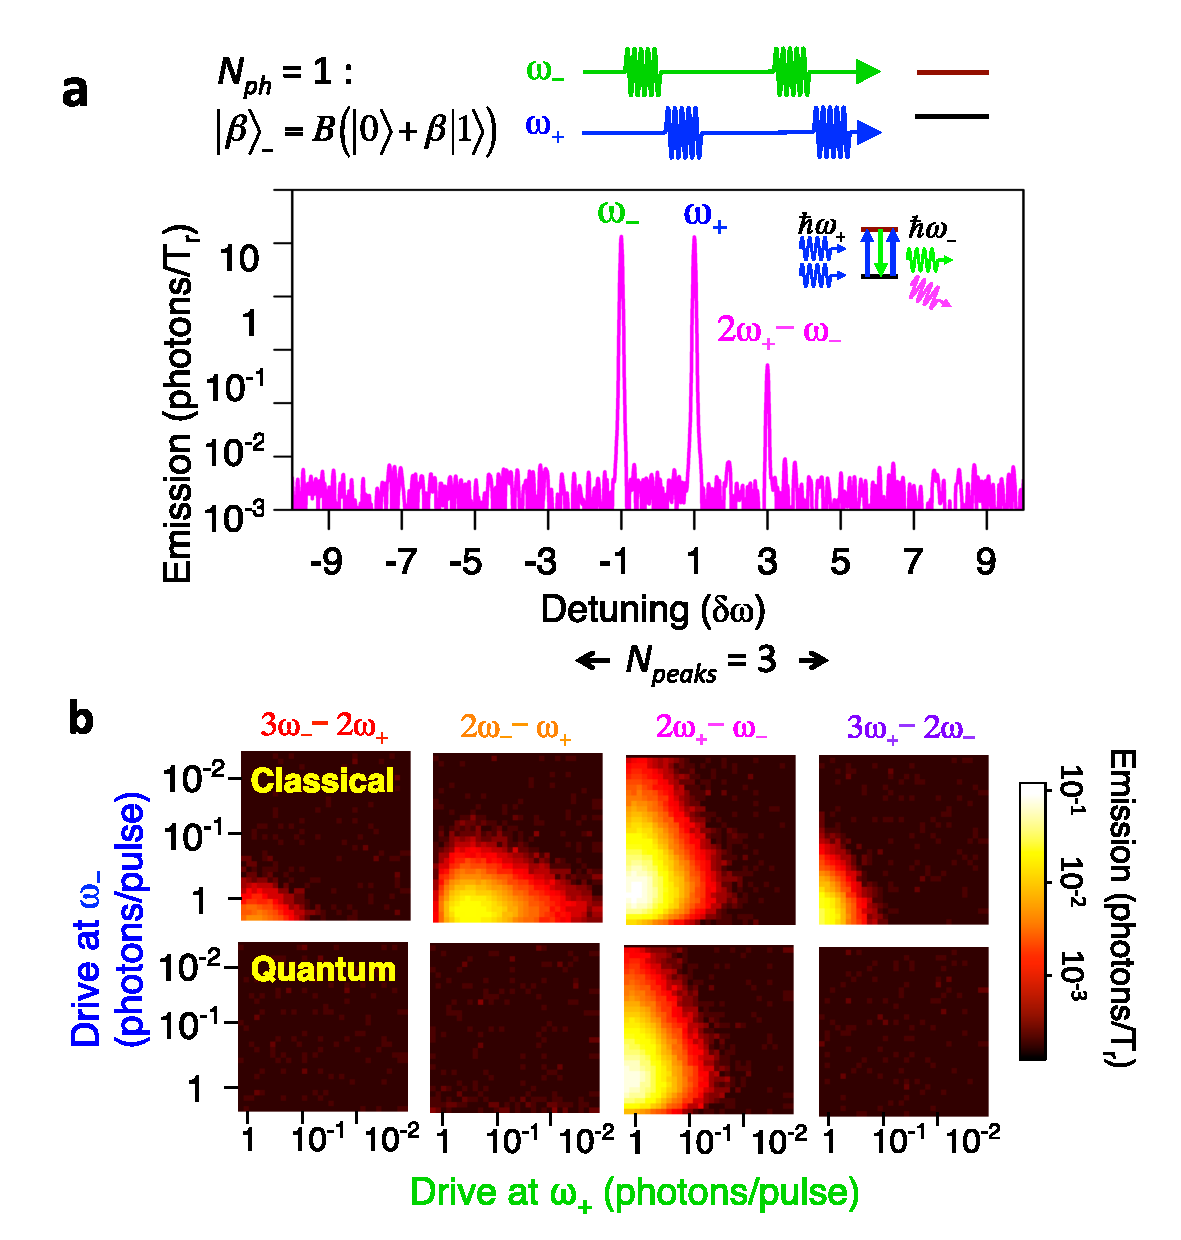
\includegraphics[width=0.8\textwidth]{Fig3_rev3.pdf}
	\caption[Квантовое волновое смешение неперекрывающихся импульсов: трехпиковый спектр.]{Квантовое волновое смешение неклассического света. (а) ---  Периодическая последовательность импульса на частоте $\omega_-$ и затем на частоте $\omega_+$ направляются на искусственный двухуровневый атом. График иллюстрирует спектр квантового волнового смешения от однофотонной когерентной суперпозиции $|\beta\rangle_-$. Единственный боковой пик возникает на частоте $2\omega_+ - \omega_-$ по причине комбинационного рассеяния фотона, $N_{ph} = 1$, от $|\beta\rangle_-$ и двух фотонов от когерентного поля второго импульса $|\alpha\rangle_+$. (b) -- Зависимость амплитуд боковых пиков при <<классическом>> смешении (в случае перекрывающихся импульсов) и квантовом смешении (случай последовательных импульсов) как функции амплитуд Раби  
		$\alpha_\pm$, выраженных в фотонах на цикл. Отчетливо наблюдается несколько боковых компонент в <<классическом>> режиме. Квантовый случай кардинально отличается полным отсутствием всех порядков, кроме пика на частоте $2\omega_+ - \omega_-$, который ведет себя практически так же как и в случае перекрывающихся импульсов. 
	}
	\label{fig: mixing_3peaks}
\end{figure}
Наблюдаемая нами в предыдущем разделе картина волнового смешения симметрична относительно частоты кубита, совпадающей с центральной частотой, причем это справедливо как для непрерывной, так и для импульсной накачки. Однако, в нашем распоряжении имеется еще один параметр, изменение которого может значительно повлиять на спектр эластичного рассеяния, изучаемый в данной работе. Этим параметром является задержка между импульсами различных частот. Можно предположить, что наиболее выразителен случай, когда задержка становится настолько большой, что первоначальные импульсы не перекрываются между собой во времени. Результат измерения эластичного спектра в этом случае приведен на Риc.~\ref{fig: mixing_mirror}а).

Введение задержки приводит к качественным изменениям в спектре: наблюдается единственная боковая спектральная компонента на частоте $\omega_{+3} = 2\omega_+-\omega_-$, если импульс на частоте $\omega_-$ предшествует импульсу на частоте $\omega_+$. Перестановка импульсов приводит к зеркально симметричному относительно центральной частоты (она же частота кубита) спектру, что опять же означает наличие единственной ненулевой боковой спектральной компоненты на частоте $\omega_{-3}$, см. Рис.~\ref{fig: mixing_mirror}. 
 
Одной из причин несимметричного спектра может являться большое различие в амплитуде полей $\Omega_+$ и $\Omega_-$, и ассимметрия может быть приписана смешению некоторого остаточного поля первого импульса со вторым импульсом. Чтобы доказать, что спектр содержит строго три пика и не больше, мы меняем амплитуды импульсов в широком диапазоне и измеряем интенсивности излучения на комбинационных частотах для случая классического и квантового смешения. Рис.~\ref{fig: mixing_3peaks}b) демонстрирует мощности излучения на боковых компонентах в различных режимах смешения: два перекрывающихся импульса\footnote{В данном разделе мы будем называть случай перекрывающихся импульсов классическим для того, чтоб отделять его от случая последовательных импульсов, где спектр более отличается от непрерывного поля. Однако, оба эффекта проявляются на квантовой двухуровневой системе и поэтому достаточно квантовые.} (верхние панели) и два последовательных импульса (нижние панели). Оба случая дают практически идентичную зависимость пика на частоте  $2\omega_+ - \omega_-$, однако остальные пики попросту отсутствуют в квантовом случае, появляясь только в классическом. 
\begin{figure}[th]
\centering
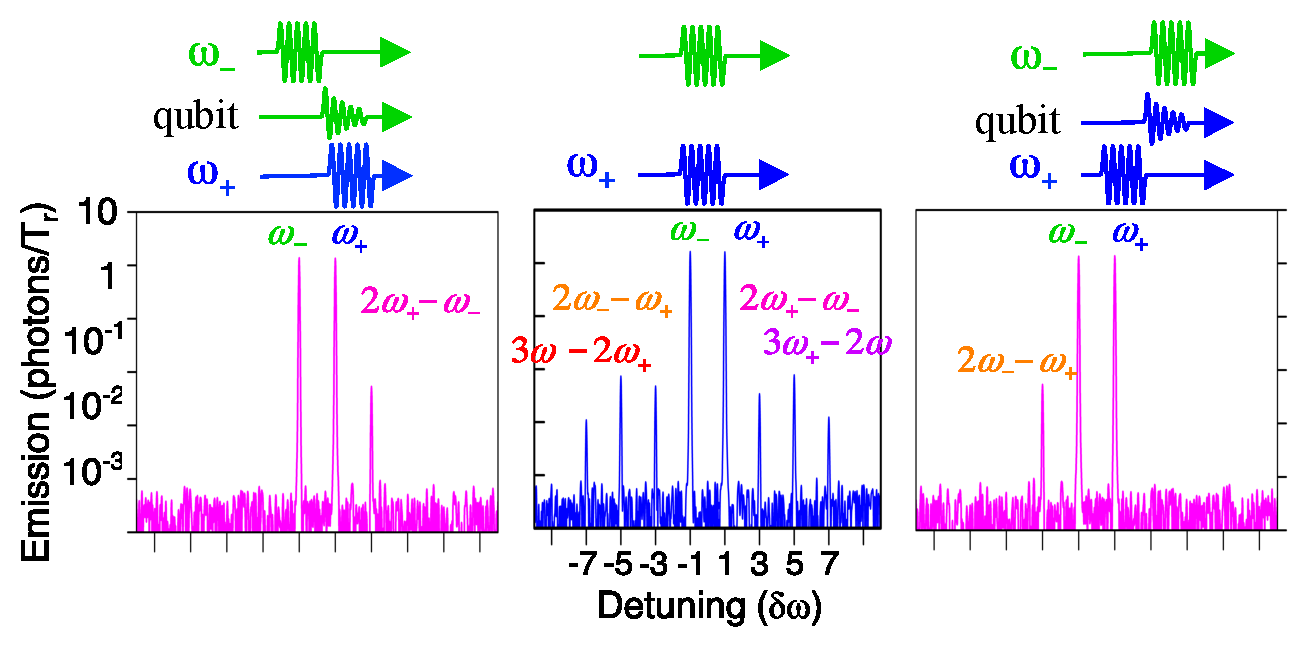
\includegraphics[width=0.9\textwidth]{QWM_slide_sqt.pdf}
\caption[Квантовое волновое смешение в зависимость от порядка импульсов]{Квантовое волновое смешение. Несимметричный трехпиковый спектр при перестановке импульсов претерпевает зеркальное отражение относительно центральной частоты. Центральный график соответствует случаю перекрывающихся импульсов, рассмотренному ранее. }
\label{fig: mixing_mirror}
\end{figure}

Наблюдаемый спектр может быть обоснован при помощи расчета оператора эволюции, подобно тому, как это было сделано в разделе \ref{sec: bessels}. Однако, прежде чем обратиться к точному теоретическому анализу наблюдаемого трехпикового спектра, полезно дополнительно подтвердить правильность предложенной качественной интерпретации. Напомним, что по нашему предположению, трехпиковый спектр объясняется тем, что двухуровневый атом <<запоминает>> единственное возбуждение, выделяя его из первого импульса, а затем происходит смешение этого возбуждения с полем из второго импульса, причем на единственно возможной частоте. Если аргументация верна, то крайне наглядно провести эксперимент по смешению на трехуровневой системе с уровнями $\ket{g}, \ket{e}, \ket{f}$, где разрешены переходы между соседними уровнями, и частоты этих переходов равны: $\omega_{ge} = \omega_{ef}$. Будем называть такую систему \textit{трехуровневой эквидистантной системой}. Очевидно, что она может запомнить два кванта возбуждения, и поэтому трехпиковый спектр должен модифицироваться в сторону увеличения числа наблюдаемых пиков. В следующем разделе мы покажем, что трехуровневую эквидистантную систему можно создать на основе того же самого потокового кубита, помещая его в определенную точку по магнитному потоку, а затем продемонстрируем как выглядит спектр квантового волнового смешения на трехуровневой эквидистантной системе. 
\section{Квантовое смешение волн на 3-уровневой системе}
Для того, чтобы определить возможность работы с потоковым кубитом в режиме квантовой трехуровневой эквидистантной системы, необходимо измерить спектр кубита в широком диапазоне. Результат измерения спектра приведен на Рис.~\ref{fig: flux_spectr_3ls}. Легко видеть, что для исследуемого потокового кубита имеется точка вблизи $\delta\Phi/\Phi_0 \approx  \pm 0.035$, где частоты переходов сравниваются, таким образом, система при ее взаимодействии с резонансной бихроматической накачкой эффективно становится трехуровневой. Направляя на кубит последовательность неперекрывающихся импульсов, рассмотренную в разделе~\ref{sec: qwm}, мы наблюдаем спектр волнового смешения, состоящий из пяти пиков, см. Рис.~\ref{fig: qwm_3ls}. 
\begin{figure}
	\centering
	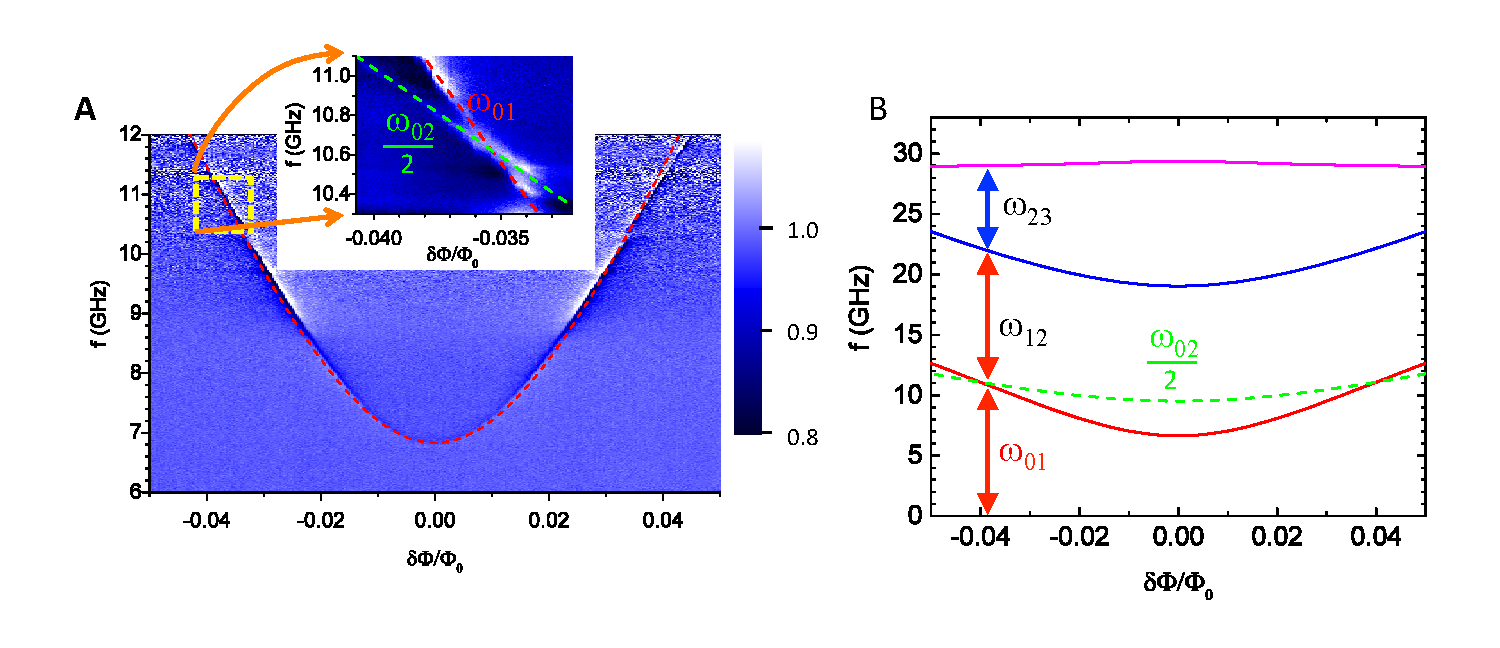
\includegraphics[width=1\textwidth]{SFig2.pdf}
	\caption[Спектр потокового кубита в широком диапазоне магнитного потока и нахождение рабочей точки, в которой кубит является трехуровневой эквидистантной системой.]{Измеренный (a) и рассчитанный (b) спектр потокового кубита в широком диапазоне магнитного потока и нахождение рабочей точки, в которой кубит является трехуровневой эквидистантной системой. Двухфотонный переход $\omega_{02}/2$ попадает в резонанс с переходом $\omega_{01}$. Отметим что за счет правил отбора в потоковом кубите в данной точке все три перехода являются разрешенными.}
	\label{fig: flux_spectr_3ls}
\end{figure}
\begin{figure}
	\centering
	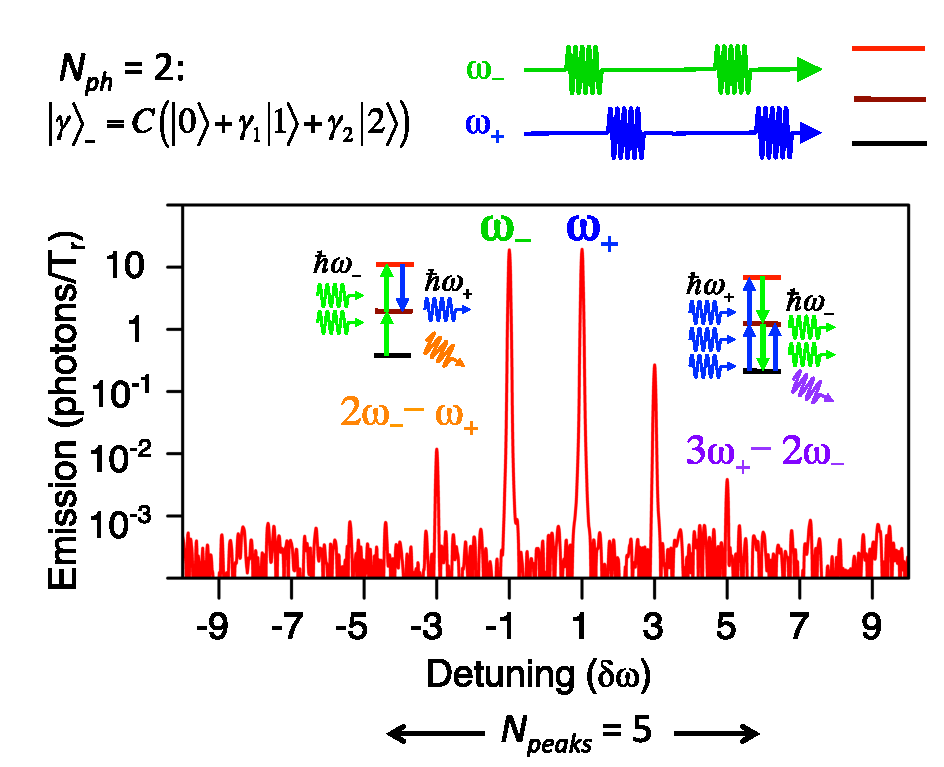
\includegraphics[width=0.6\textwidth]{Fig4_rev3.pdf}
	\caption[Спектр квантового волнового смешения на трехуровневой эквидистантной системе.]{Квантовое волновое смешение на трехуровневой эквидистантной системе с вовлечением двухфотонных состояний. Спектр смешения на трехуровневом атоме содержит три боковых пика, что является результатом отображения состояния системы с двумя возбуждениями $|\gamma\rangle_-$ ($N_{ph} = 2$). Сравнивая с Рис.~\ref{fig: mixing_3peaks}, дополнительный пик на частоте $3\omega_+ - 2\omega_-$ соответствуют двухфотонному излучению из состояния $|\gamma\rangle_-$. Процесс поглощения двух фотонов выражается в наличии пика на частоте $2\omega_- - 2\omega_+$, что завершает иллюстрацию всех разрешенных процессов при помощи спектра волнового смешения. Важно, что эксперимент отличает многофотонный случай на Рис.~\ref{fig: Bessels} ($N_{ph} = \infty$), однофотонное ($N_{ph} = 1$) и двухфотонное ($N_{ph} = 2$) состояния суперпозиции.}
	\label{fig: qwm_3ls}
\end{figure}
Поскольку вновь появившиеся пики возникли на частотах $\omega_{+5} = 3\omega_+-2\omega_-$ и $\omega_{-3} = 2\omega_--\omega_+$ --- на тех и только на тех частотах, которые вовлекают два фотона на частоте первоначального импульса $\omega_-$ --- то мы убеждаемся, что добавление третьего уровня и второго возбуждения в атом меняет картину смешения. Это является еще одним аргументом в пользу инерпретации спектра в качестве <<отпечатка>> различных многофотонных состояний, присутствующих в системе. Завершая обзор экспериментальных результатов в данной части диссертационной работы, приведем также сравнительную картину режимов волнового смешения в зависимости от угла поворота импульсов $\Omega\delta t$, см. Рис.~\ref{fig: qwm_all}. 
\begin{figure}
	\centering
	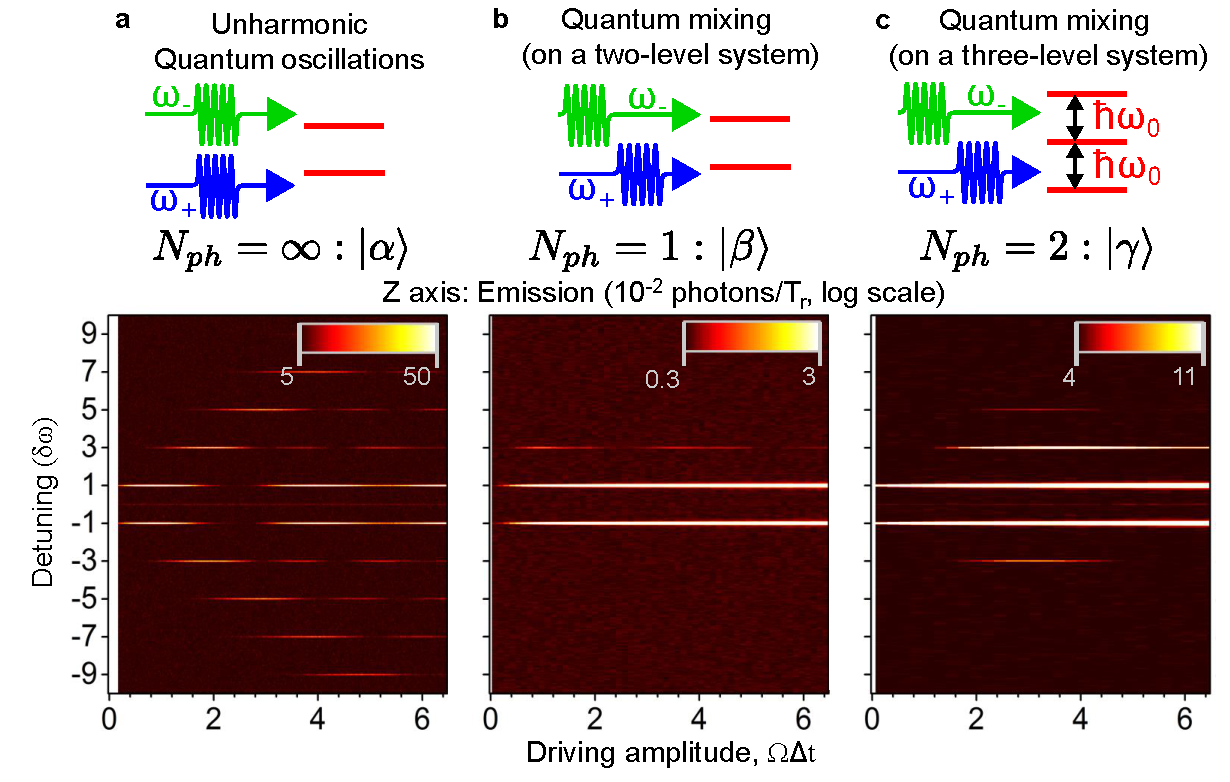
\includegraphics[width=0.9\textwidth]{Fig5_rev3.pdf}
	\caption[Сравнение различных режимов волнового смешения]{Различные режимы волнового смешения, представленные в виде зависимости от угла поворота импульсов. a) Бесселевское разложение осцилляций Раби в классическом волновом смешении на искусственном атоме. b) Квантовое волновое смешение на двухуровневой системе. Наблюдается одиночный боковой пик. c), Квантовое смешение на 3-уровневой системе. Два дополнительных боковых пика являются проявлением возможности возбуждения трехуровневой системы двумя фотонами, взятыми из начального импульса. }
	\label{fig: qwm_all}
\end{figure}
Мы установили, что спектр эластичного рассеяния при квантовом волновом смешении определяется свойствами как квантовой системы, на которой происходит смешение, так и временной диаграммой поля (говоря иначе --- конфигурацией возбуждающих бихроматических импульсов), распространяющегося в волноводе, где находится квантовая система. Для того, чтобы строго объяснить особенности спектров, проведем аналитический расчет интенсивности эластичных компонент поля. Это можно сделать на основе разобранного в разделе~\ref{sec: bessels} формализма. Аналитическому расчету интенсивности эластичных боковых компонент посвящается следующий раздел данной диссертационной работы.  
\section{Аналитический расчет спектров в представлении вторичного квантования}
Для того, чтобы получить спектр эластичного рассеяния для последовательностей неперекрывающихся импульсов, рассмотрим эволюцию под действием гамильтониана, записанного в представлении взаимодействия. Прожде всего отметим, что число мод в волноводе очень велико, но нас будет интересовать спектр от двух периодических сигналов, поэтому мы можем свести задачу к взаимодействию кубита поочередно с модами на частотах $\omega_-, \omega_+$. Поэтому достаточно использовать гамильтониан \eqref{Hqintb} и соответствующий ему оператор эволюции \eqref{u1}. 
\subsection{Случай двухуровневой системы}
Мы рассмотрим эволюцию под действием двух последовательных импульсов на частотах $\omega_-$ и $\omega_+$. Для удобства, мы возьмем начальное состояние в виде $\ket{0, \alpha_-, \alpha_+}$, но будем считать что операторы эволюции, определенные в уравнении~(\ref{u1}) действуют друг за другом в течении короткого времени. Иными словами, мы считаем что связь с каждой из мод включается только при прохождении соответствующего импульса через кубит. Для дальнейшего использования введем операторы:
\begin{equation}
\hat{\beta}^+_{\pm} = \beta_\pm a_\pm b^+_\pm (a^\dag_\pm a_\pm)^{-1/2}\approx \beta_{\pm}b^+_{\pm},
\label{beta_op}
\end{equation} 
где $\beta_\pm = \tan(\theta_\pm/2)$, $B_\pm = \sqrt{1+\beta_\pm^2}$, $\theta_- = 2g_- \alpha_- (t'-t)$, $\theta_+ = 2g_- \alpha_-(t''-t')$. Приближенное равенство в \eqref{beta_op} справедливо при условии $\alpha_{\pm} \gg 1$. С помощью этих операторов удобно записывать операторы эволюции. Первый импульс на частоте $\omega_-$ приводит к излучению поля в состоянии суперпозиции вакуума и одиночного фотона $|\beta\rangle_- = B_-(1-\hat{\beta}_-^+)\ket{0}$, что описывается эволюцией:
\begin{equation}
	U(t^\prime,t)\ket{0,\alpha_-,\alpha_+} =  B_- (1 - \beta_- b^+_-)\ket{0,\alpha_-,\alpha_+}=\ket{\beta_-}\otimes\ket{\alpha_-,\alpha_+},
\end{equation}
и это состояние мы обозначим $\ket{\beta_-,\alpha_-,\alpha_+}$. Затем это состояние эволюционирует при взаимодействии со вторым импульсом, представляемым когерентным состоянием $|\alpha\rangle_+$. Мы покажем, что среди всех процессов третьего или более высокого порядка, единственный нетривиальный вклад в среднее поле, приводящий к появлению излучения на новой частоте, дается слагаемым вида $A^-_{3} b^+_3 = a_- a^\dag_+ a_- b^-_3$, потому как всего один фотон может быть испущен на частоте $|\beta\rangle_-$. Все другие процессы оказываются запрещенными из-за того, что только одиночное возбуждение остается в кубите после взаимодействия с первым импульсом, что приводит к недостатку фотонов на частоте $\omega_-$. В итоге, единичный фотон может излучаться только на частоте $2\omega_+ - \omega_- = \omega_d + 3\delta\omega$. 

Эволюция под действием второго импульса записывается как 
\begin{equation}
	U(t',t'') |\beta_-,\alpha_-,\alpha_+\rangle \approx B_+ \bigg(1 + \hat{\beta}^-_+ - \hat{\beta}^+_+\bigg)  |\beta_-,\alpha_-,\alpha_+\rangle, 
	\label{Utt}
\end{equation}
Последнее равенство можно упростить: 
\begin{equation}
	U(t',t'') |\beta_-,\alpha_-,\alpha_+\rangle \approx B_+ B_- \Big(1 - \hat\beta^+_+  - \hat\beta^+_- - \hat\beta^-_+ \hat\beta^+_-\Big)|0,\alpha_-,\alpha_+\rangle, 
\end{equation}
также отметим что $\hat\beta^-_\pm =(\hat\beta^+_\pm)^\dag$. Как показано ранее, излучаемое поле на частоте $\omega_p$ пропорционально среднему от оператора уничтожения:
\begin{equation}
	\braket{b^-_p} = \braket{0,\alpha_-,\alpha_+|U^\dag(t',t)U^\dag(t'',t') b^-_p U(t'',t')U(t',t)|0, \alpha_-, \alpha_+}.
\end{equation}
Мы хотим сосчитать все фазовые факторы вида $e^{\pm i\delta\omega t}$, появляющиеся от операторов $\hat{\beta}^{\pm}_{\pm}$ и потом определить, для какого $p$ оператор $b^-_{p}$ усреднение по состоянию даст константу, не обращающуюся в ноль после усреднения по времени. Именно здесь и определятся частоты излучаемого поля в рамках когерентного рассеяния. После подстановки, мы получаем:
\begin{equation}
	\begin{split}
	\braket{b^-_p} = B_-^2B_+^2\bra{0,\alpha_-,\alpha_+}\big(
		&-\underbrace{b^-_p\hat{\beta}^+_+}_{e^{i\delta t}}
		-\underbrace{b^-_p\hat{\beta}^+_- }_{e^{-i\delta t}} \\
		&+\underbrace{\hat{\beta}^-_- \hat{\beta}^+_+ b^-_p  \hat{\beta}^+_-}_{e^{i\delta t}} 
		+\underbrace{\hat{\beta}^+_+ \hat{\beta}^-_-b^-_p\hat{\beta}^+_+  }_{e^{3i\delta t}}
		\big) \ket{0,\alpha_-,\alpha_+}
	\label{b_dag}
	\end{split}
\end{equation}
Мы видим, что среди всех членов \eqref{b_dag}, только последнее слагаемое создает поле на боковой частоте, потому как
\begin{equation}
	B_+^2 B_-^2\braket{\hat{\beta}^+_+ \hat{\beta}^-_-b^-_3\hat{\beta}^+_+ } = B_+^2 B_-^2\beta^2_+\beta_-\braket{\alpha_-,\alpha_+| \frac{A^-_{3}}{a^\dagger_+ a_+(a^\dagger_- a_-)^{1/2}}|\alpha_-,\alpha_+}
\end{equation}
отлично от нуля. 
Окончательно, среднее значение оператора находим как 
\begin{equation}
	\langle b^-_3 \rangle \approx B_+^2 B_-^2 \beta_+^2\beta_- = \frac{1}{2}\sin^2\left[\frac{\Omega_+}{2} (t''-t')\right]\sin\left[\Omega_- (t'-t)\right],
\end{equation}
\subsection{Случай трехуровневой системы}
По аналогии с расчетом, представленным в предыдущем разделе, можно вычислить спектр смешения на эквидистантной трехуровневой системе. Для 
\section{Численный расчет импульсной динамики}


